\documentclass[12pt]{article}
\usepackage{fancyhdr}
\usepackage{datetime}
\usepackage{graphicx}
\usepackage{amsmath}
%\usepackage{showframe}

%custom variables
\newdate{date}{16}{09}{2016}
\newcommand{\hwNum}{1}
\newcommand{\type}{Lab No.}
\graphicspath{ {images/} }


%header
\pagestyle{fancy}
\lhead{Daniel Andronov}
\chead{\thepage}
\rhead{\type{} \hwNum{}}
\cfoot{\thepage}

\fancyheadoffset[LO,RE]{1pt}
\fancyheadoffset[RO,LE]{1pt}

%titlepage
\title{\type{} \hwNum{}}
\author{Daniel Andronov}
\date{\displaydate{date}}

%addition settings
\topmargin=-0.45in
\evensidemargin=0in
\oddsidemargin=0in
\textwidth=6.5in
\textheight=9.0in
\headsep=0.25in

\begin{document}
\maketitle
\newpage

\section{Questions from Seciont 2.3}


\paragraph{Problem 1}
During the first iteration, the total load, $L$ on node 0 is \\
\begin{align}
 L & = \frac{ R_{agg} }{Link Cap }  = \frac{  4 \times R_a }{1 Mb/s }\\
&   = \frac{ 4\times R_p \times F_{on} }{1 Mb/s } = \frac{500 Kb/s}{1Mb/s} = 0.5 
\end{align}
So, the total load on node 0 is 0.5. However, it is still possible to incurr packet loss if all nodes transmit at once, which has a probability of $1/2^4$ or 6.25\% chance of occuring. 

\paragraph{Problem 2}
I first observed packet loss occuring during the third iteration when the load on node0 was 60\%. Even though the load is much less than one, if all nodes transmit at once then the node will have to deal with traffic incoming at 1.2Mb/s, which is over the link capacity. 

\paragraph{Problem 3 \& 5}
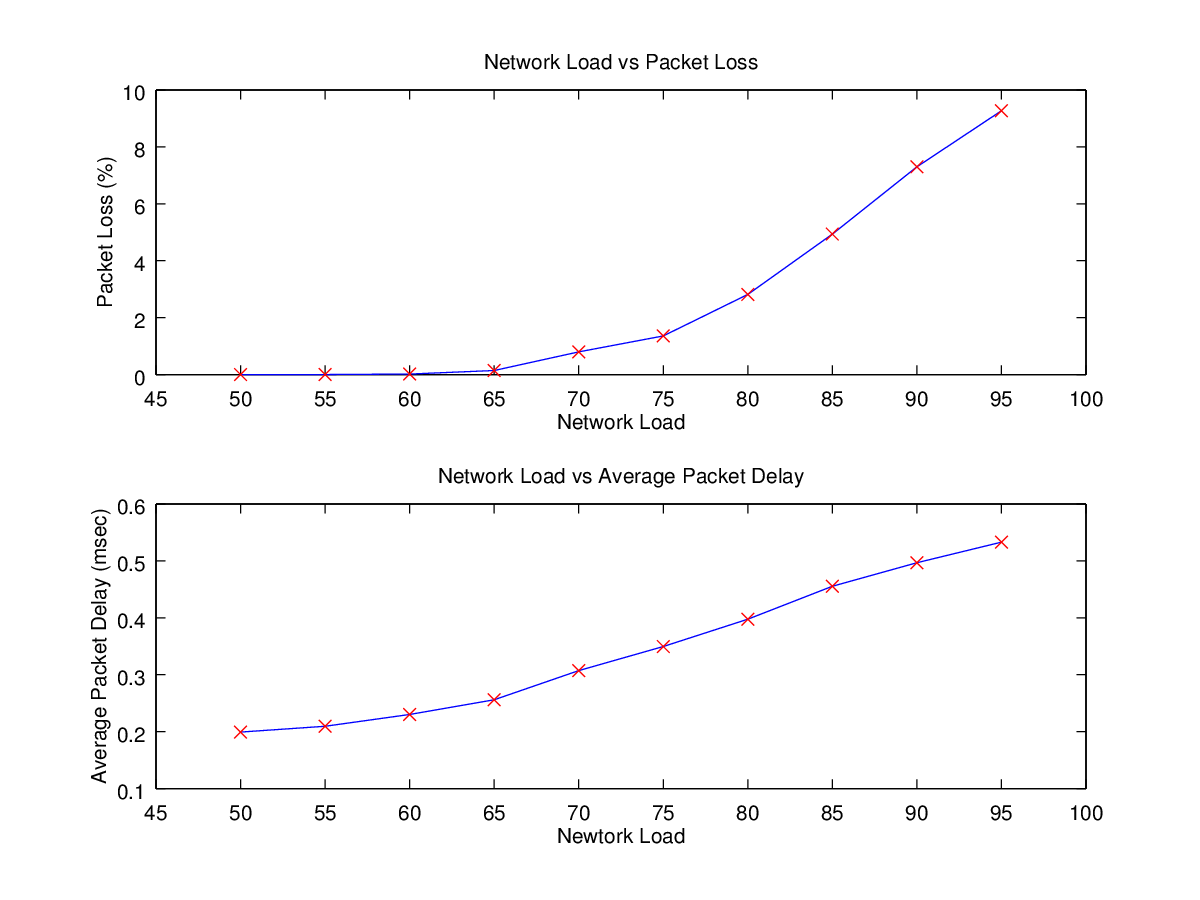
\includegraphics{fig}

\end{document}
This is never printed